\subsection{Background}

As an alternative to metropolitan statistical areas (or Core Based Statistical Areas), many researchers use Commuting Zones because they cover the entire country and group counties based on commuting flows, which is a measure of labor market integration. However, few researchers are familiar with the underlying methodology. To that end, this section describes the commuting zone  methodology, as developed by TS1996. 

The methodology was  originally developed in \citet{TK1987}, but the 1996 paper is much more widely cited. The Economic Research Service (ERS), an agency under the Department of Agriculture for which this methodology was developed, distributes commuting zone definitions on its website. Commuting Zones are especially relevant for the economic analysis of rural areas because the include all counties, not just urban counties. ERS also distributes a version of Commuting Zones based on 2000 data. For a research into extending the time series of Commuting Zones and further background on TS1996, see \cite{FowlerRhubartJensen2016}.

To define an exhaustive classification of counties, TS1996 calculated a dissimilarity matrix $D$, where an entry $D_{ij}$ is the dissimilarity of county $i$ from county $j$, calculated as below:\footnote{Due to computational constraints at the time, TS1996 broke the country into six overlapping regions: Northeast, Southeast, Midwest, Southwest, Central and West, calculating a separate distance matrix for each region.}
\begin{equation}\label{eqn:distance}
D_{ij} = 1- P_{ij} = 1- \frac{f_{ij} + f_{ji}}{\min(rlf_i,rlf_j)}
\end{equation}
where $f_{ij}$ is the number of commuters who live in $i$ and work in $j$, and $rlf_i = \sum_{j} f_{ij}$ (including $f_{ii}$) is the resident workforce. The data used in TS1996 to estimate the flows is from the \mc{1990 Journey to Work data}{LV: Reference/bibliographic entry}, released from the 1990 Census. Other releases based on data from the 1980 and 2000 Censuses are also available.\footnote{These CZ definitions are available at \url{http://www.ers.usda.gov/data-products/commuting-zones-and-labor-market-areas.aspx}}
After constructing this dissimilarity matrix, they use it as the input into an average-linkage hierarchical clustering algorithm (\mc{PROC CLUSTER in SAS}{LV: Cite the online PDF explaining the procedure for SAS 9.2, see if you can find the proper quote for SAS 6.12, which was likely the version they used - might be in the Census library, or even in LEHD}). They allow clusters to form that are no higher than a `height' of 0.98.\footnote{In the average-linkage clustering algorithm, the height (or distance) between clusters is given by the following formula:
\[
D_{KL} = \frac{1}{N_K N_L} \sum_{i \in C_k} \sum_{j \in C_L} d(x_i,x_j)
\]
That is, the distance between two clusters is the average of the pair-wise distances between each component of the two clusters. Therefore, that implies no clusters were merged such that $D_{KL}>0.98$.  (\href{https://support.sas.com/documentation/cdl/en/statug/63347/HTML/default/viewer.htm\#cluster_toc.htm}{SAS Manual, version 9.2})} Additionally, because they cluster separately for region, and there are a number of states that are in multiple regions, they manually reconcile these competing cluster definitions, but do not provide their methodology for this reconciliation in the paper. Finally, they mention that they do perform a national analysis, but do not report the results.

We illustrate the process in Appendix Figure \ref{fig:caliclusters}, which shows how the counties are clustered together for California. In the top left-hand corner, only a few counties have joined at a height of 0.8. As we increase the height of allowable clusters from 0.8 to 0.88, more counties are joined together to make clusters, and the same is true when increasing the height to 0.96. Finally, at a height of 1, almost all the counties have merged together and there is one large cluster and a few much smaller clusters.

\subsection{Replicating Tolbert and Sizer's Definitions}

% Source program: /modules/module_mapjtw1990.sas
% Last updated:


%%%%% COMMUTING ZONES
\begin{figure}[th]
\caption{Replication of Commuting Zones from TS1996: County Mapping}
%\begin{subfigure}[t]{0.5\textwidth}
\begin{tabular}{cc}
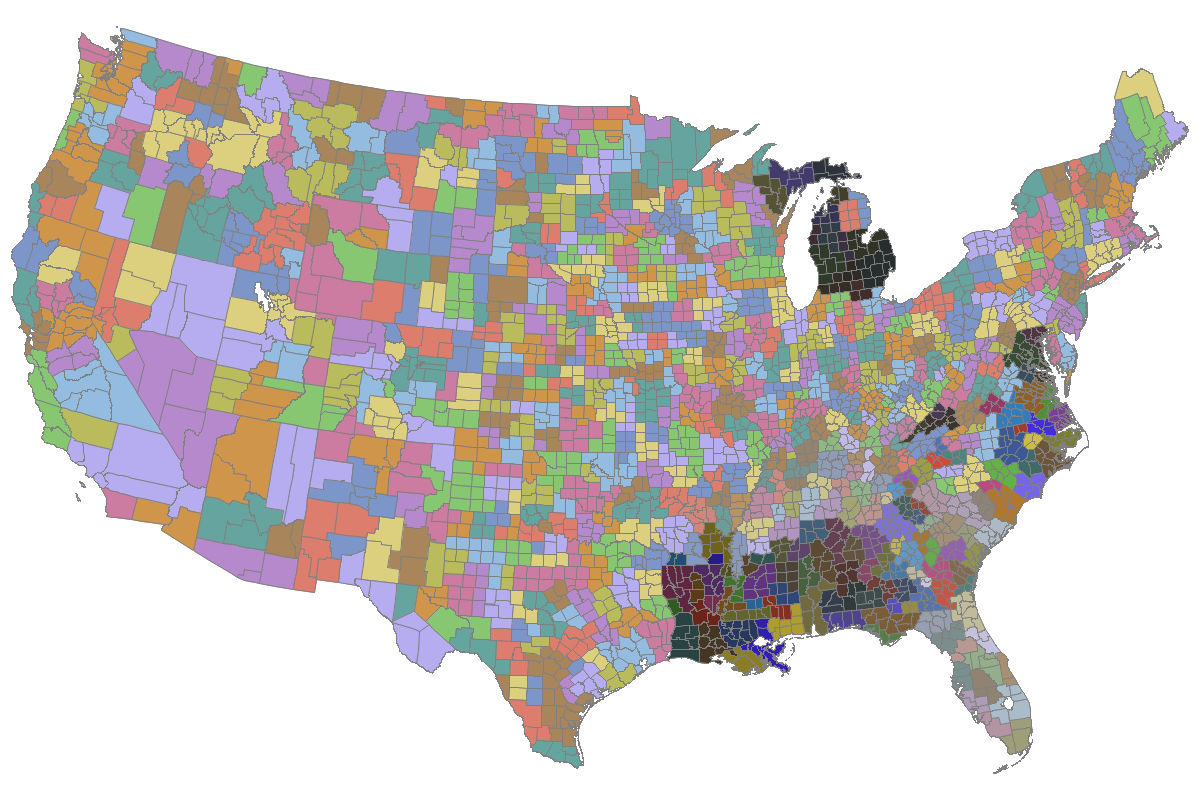
\includegraphics[width=.48\textwidth]{./figures/commutingzones.png}
&
%\caption{Tolbert and Sizer's Commuting Zones}
%\end{subfigure}
%\begin{subfigure}[t]{0.5\textwidth}
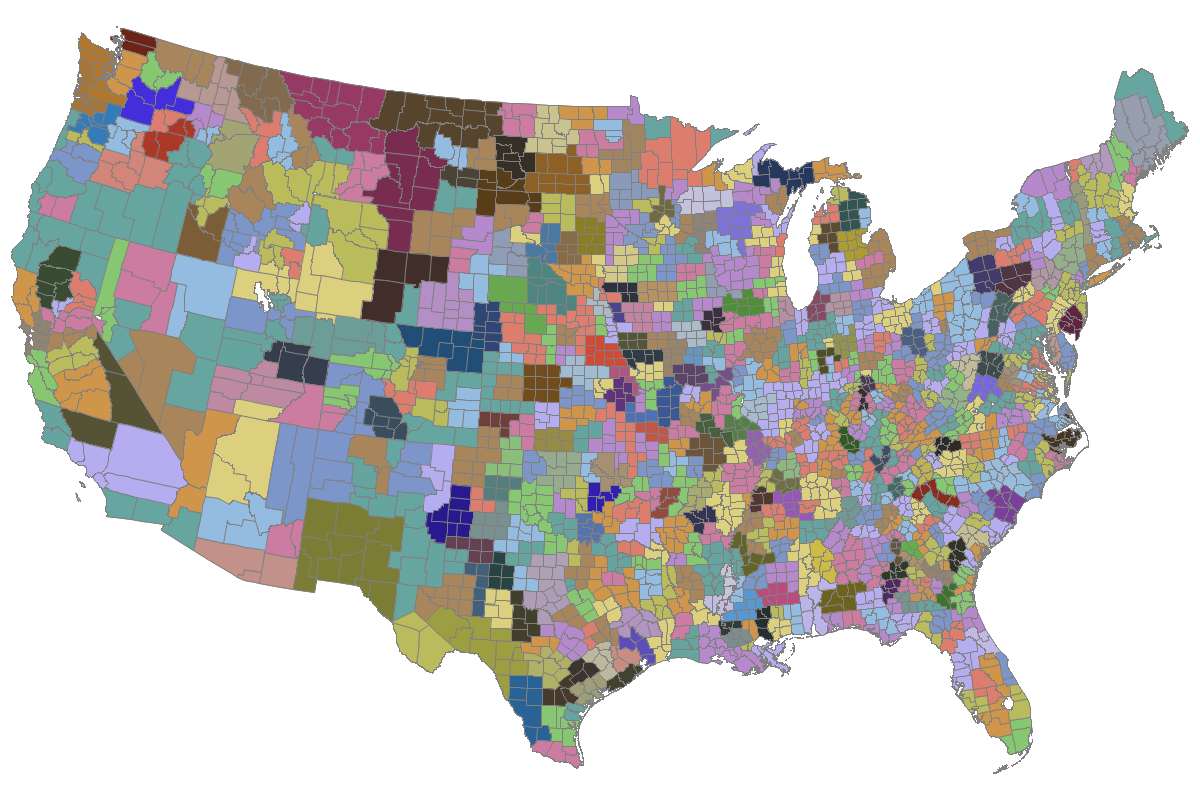
\includegraphics[width=.48\textwidth]{./figures/replication.png}
\\
{Commuting Zones from TS1996: TS1990}
&
{Replication of Commuting Zones: FKV1990}
\\
\end{tabular}
\label{fig:czmaps}
\end{figure}


% source: name of SAS program
% Last updated:

\begin{table}\centering
\caption{Replication of TS1990 Commuting Zones: Summary Statistics \label{tab:replication}}
\begin{tabular}{lcc}
\hline\hline
       & TS1990 &  FKV1990  \\
       \hline
Mean Cluster Size &  4.24  & 4.16 \\
Median Cluster Size & 4 & 4 \\
Number of Clusters & 741 & 755  \\
Number of Singletons & 62 &  12 \\
Share of Population Mis-matched & \multicolumn{2}{c}{0.17}\\
\hline
\multicolumn{3}{p{4in}}{\footnotesize \textit{Notes}: Both TS1990 and FKV1990 are based on JTW tabulations from the 1990 Census. Summary statistics for TS1990 are from Table 8 of TS.}\\
\end{tabular}
\end{table}



In order to replicate the clustering result in TS1996, which we refer to as TS1990, we use the 1990 Census JTW data and the methodology described above.\footnote{Rather than splitting the country into separate regions, we perform our clustering at the national level, because it is computationally feasible to do so. We attempted to replicate their methodology at the regional level, but were unable to determine how they reconciled competing definitions across regions. \cite{FowlerRhubartJensen2016} document the expert review process in the original Commuting Zone delineations.} 
Our analysis showed that using a height cutoff of 0.9365 gives us results that are closest to the TS1990 mapping. We refer to the resulting clusters as FKV1990. Figure \ref{fig:czmaps} shows a visual comparison of TS1990 and FKV1990 communting zones, while Table \ref{tab:replication} shows summary statistics of TS1990 and FKV1990. There are 739 clusters in FKV1990, compared with  741 clusters in TS1990. In both sets, the average number of counties per cluster is 4.24, while the median is 4.

We also calculate two similarity measures between the clusters: for each county, the share of counties in our clusters that are in the same TS1990 commuting zone; and the share of counties in a TS1990 commuting zone are in the same cluster (unweighted). Both metrics are  over 80\%. Overall, we conclude that while not exactly identical, the FKV1990 replication of TS1990 is reasonably close.\mc{}{MK: Are these job weighted?}

